\begin{figure}[!htbp]
        \centering
        \begin{subfigure}[b]{0.49\textwidth}
                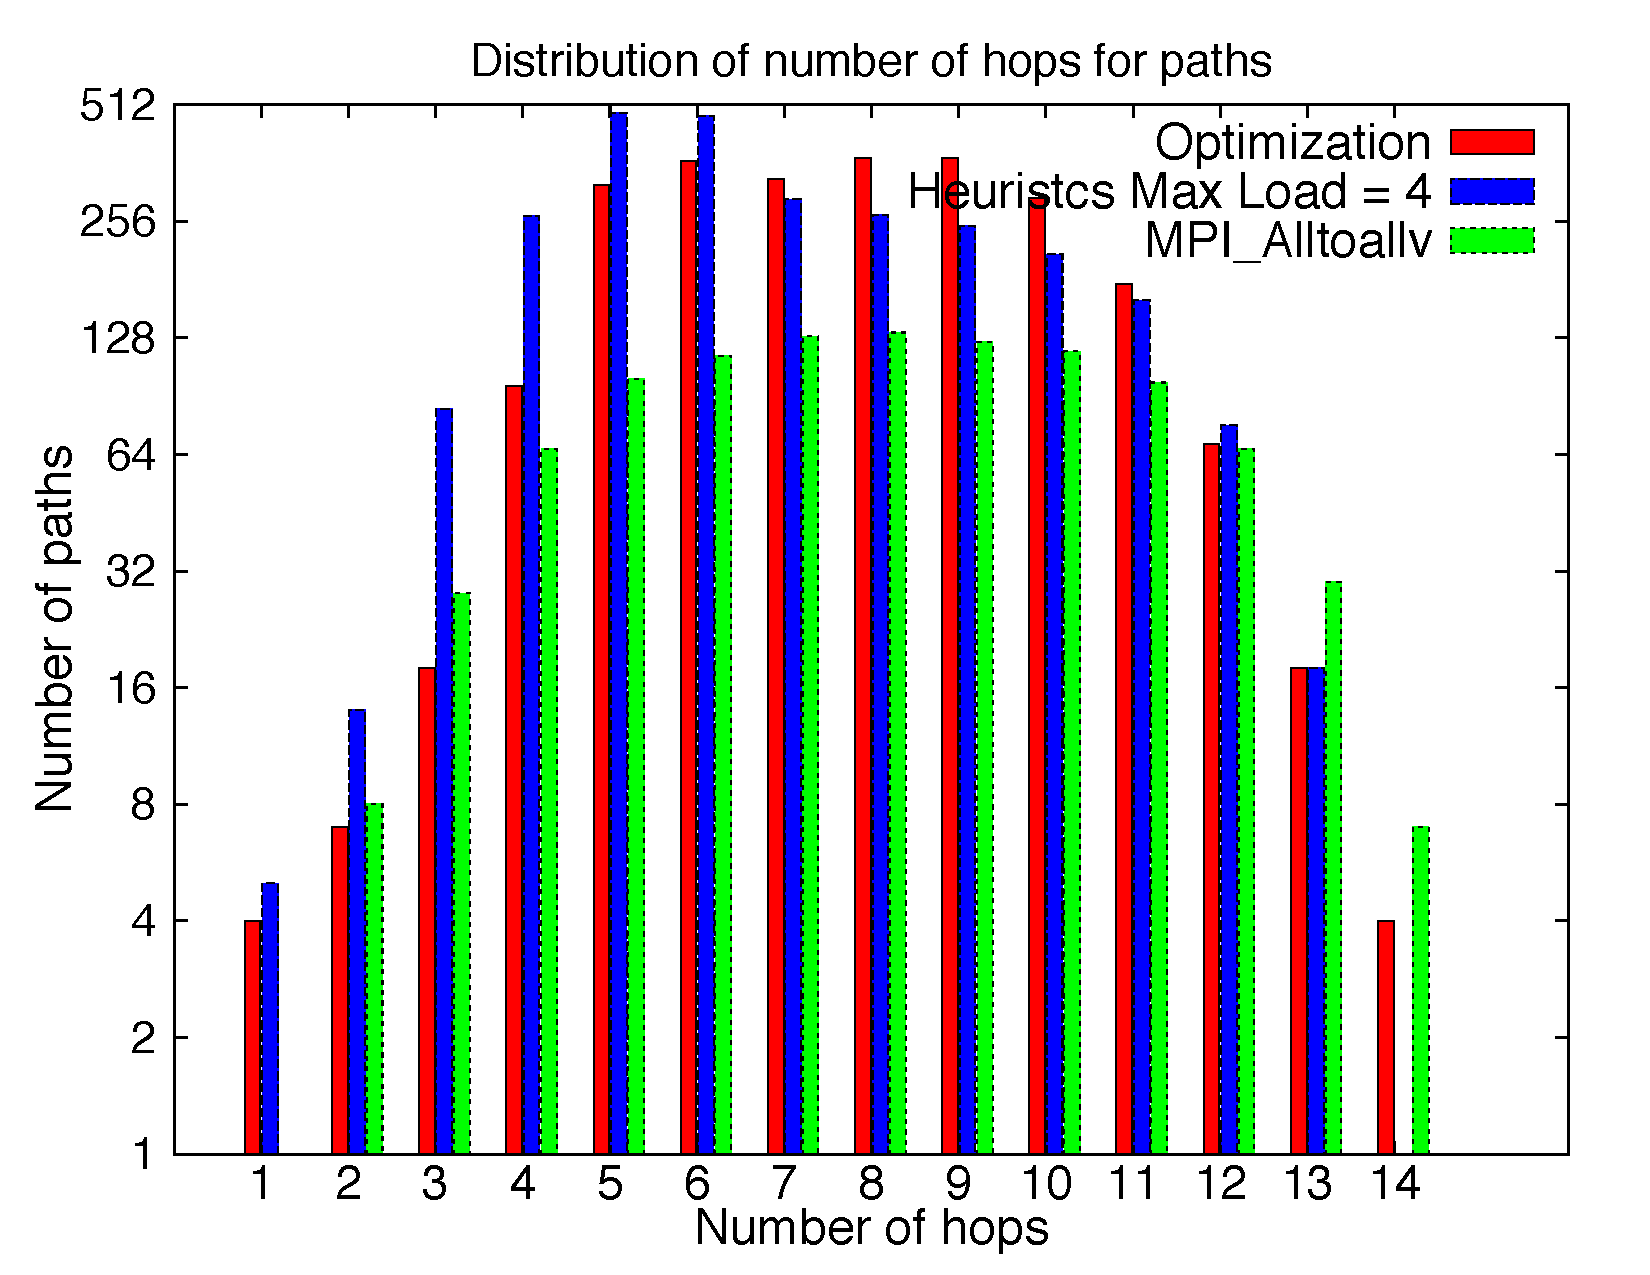
\includegraphics[width=\textwidth]{report_figures/constantr/87_2048/hop_histo.pdf}
                \caption{Distribution of number of hops over paths}
                \label{fig:87_2048_hop}
        \end{subfigure}%
        ~ %add desired spacing between images, e. g. ~, \quad, \qquad, \hfill etc.
          %(or a blank line to force the subfigure onto a new line)
        \begin{subfigure}[b]{0.49\textwidth}
                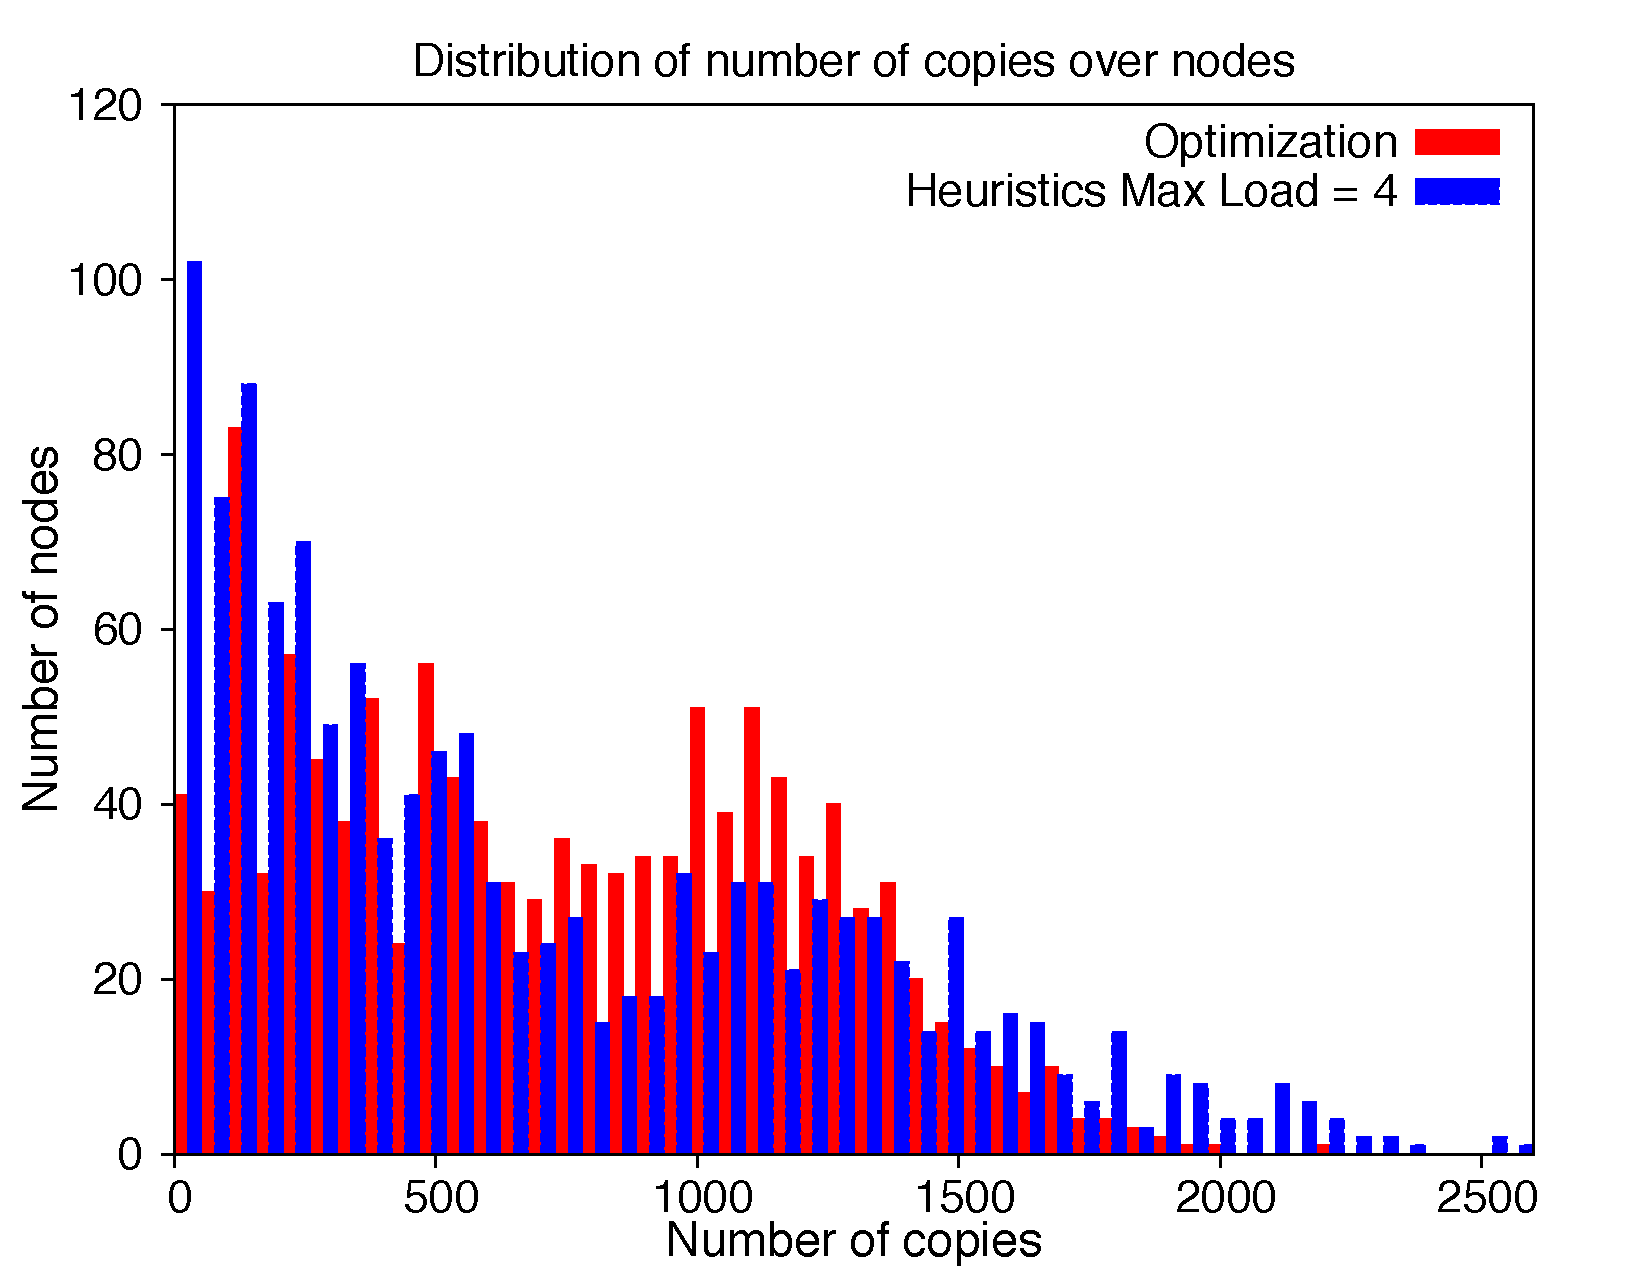
\includegraphics[width=\textwidth]{report_figures/constantr/87_2048/copy_histo.pdf}
                \caption{Distribution of number of copies over nodes}
                \label{fig:87_2048_copy}
        \end{subfigure}
        ~ %add desired spacing between images, e. g. ~, \quad, \qquad, \hfill etc.
          %(or a blank line to force the subfigure onto a new line)
        \begin{subfigure}[b]{0.49\textwidth}
                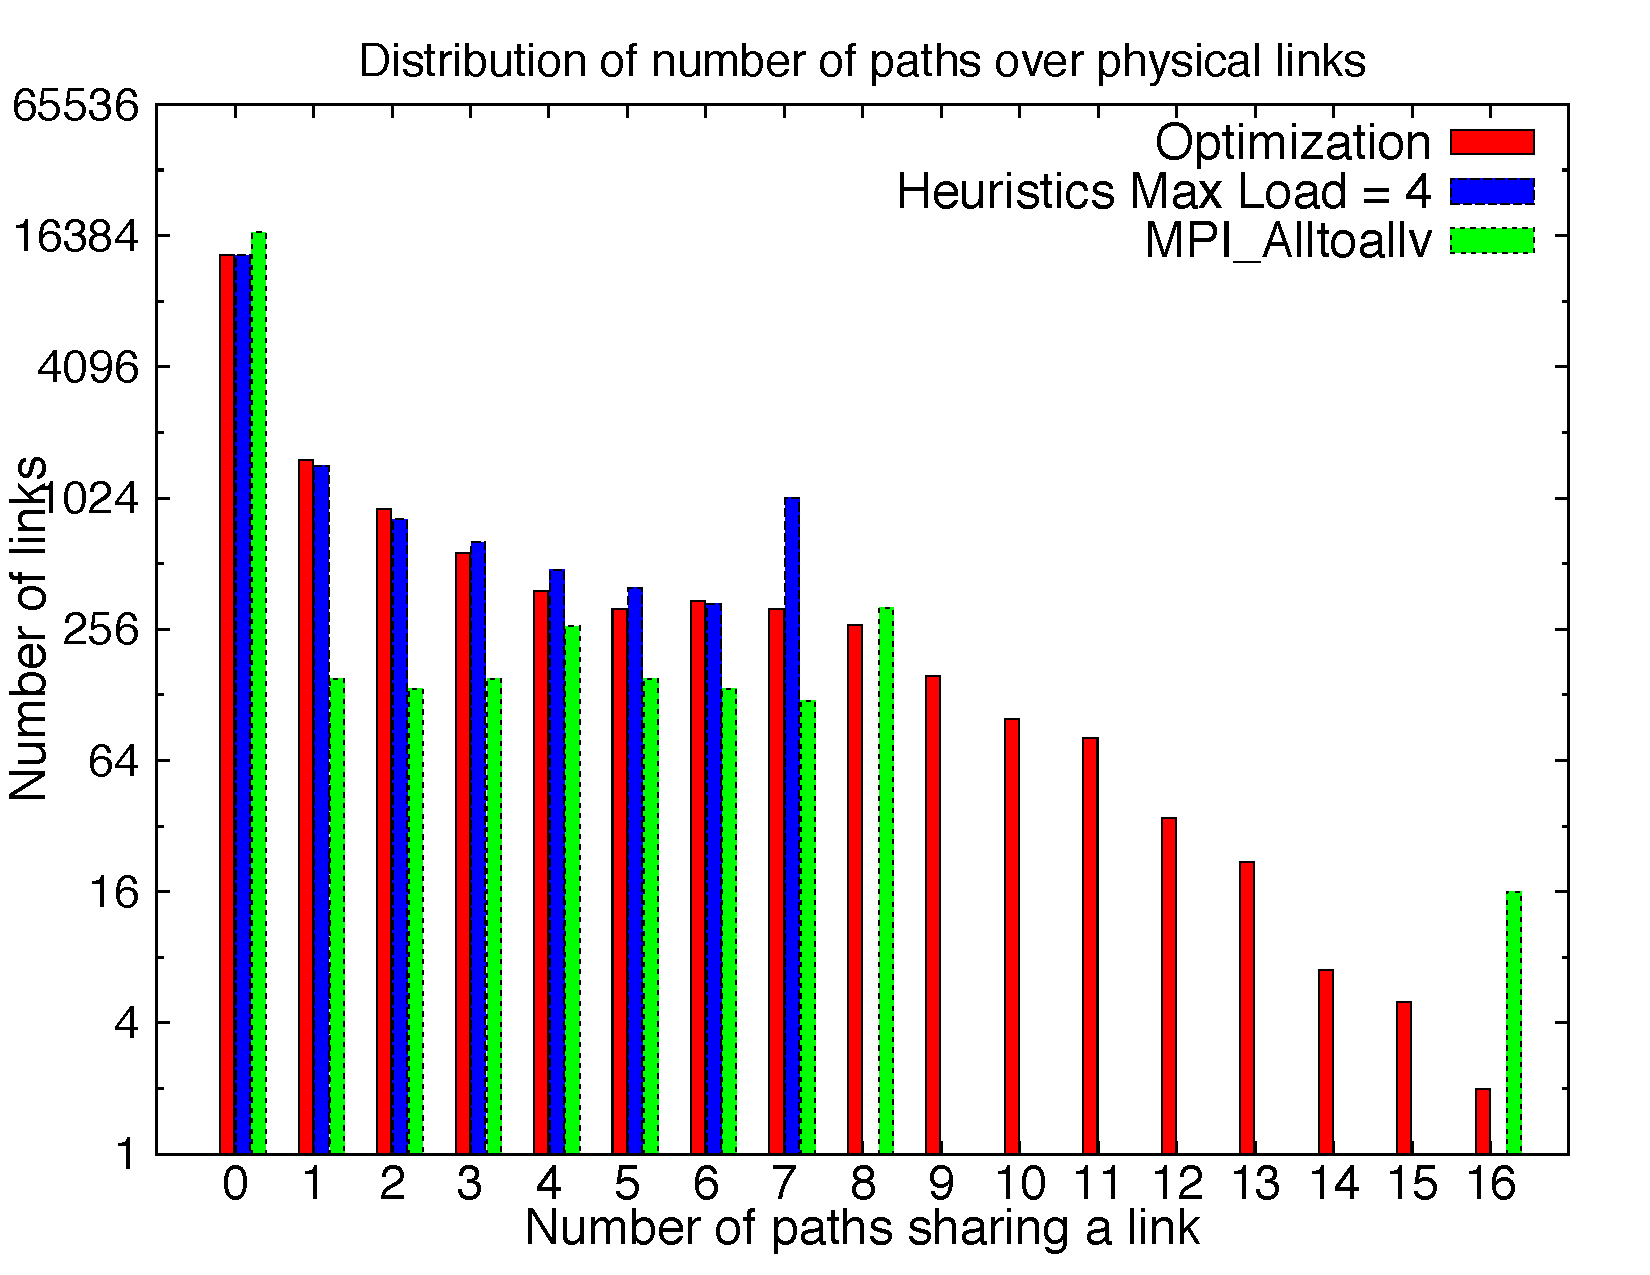
\includegraphics[width=\textwidth]{report_figures/constantr/87_2048/loadpath_histo.pdf}
                \caption{Distribution of number of paths over physicallinks}
                \label{fig:87_2048_loadpath}
        \end{subfigure}
        ~ %add desired spacing between images, e. g. ~, \quad, \qquad, \hfill etc.
          %(or a blank line to force the subfigure onto a new line)
        \begin{subfigure}[b]{0.49\textwidth}
                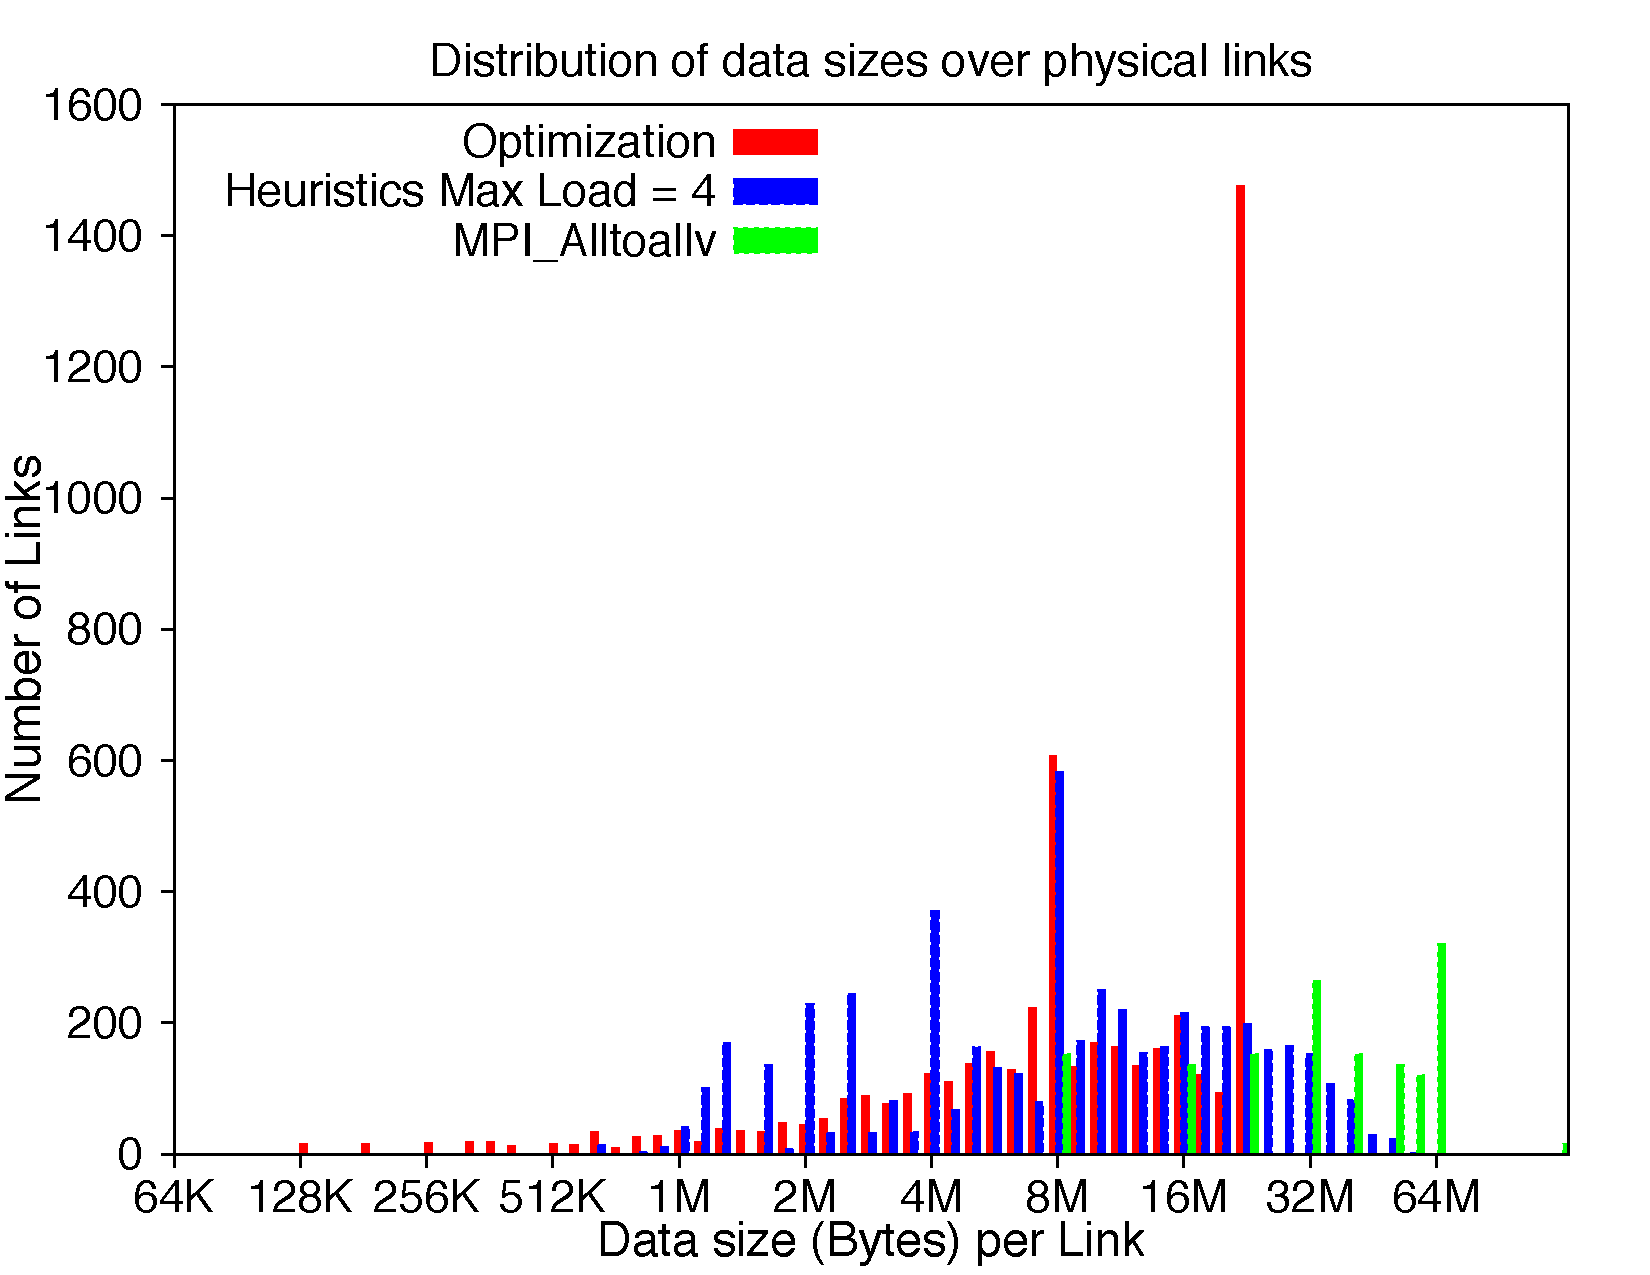
\includegraphics[width=\textwidth]{report_figures/constantr/87_2048/loaddata_histo.pdf}
                \caption{Distribution of total data size over physical links}
                \label{fig:87_2048_loaddata}
        \end{subfigure}
        ~ %add desired spacing between images, e. g. ~, \quad, \qquad, \hfill etc.
          %(or a blank line to force the subfigure onto a new line)
        \begin{subfigure}[b]{0.49\textwidth}
                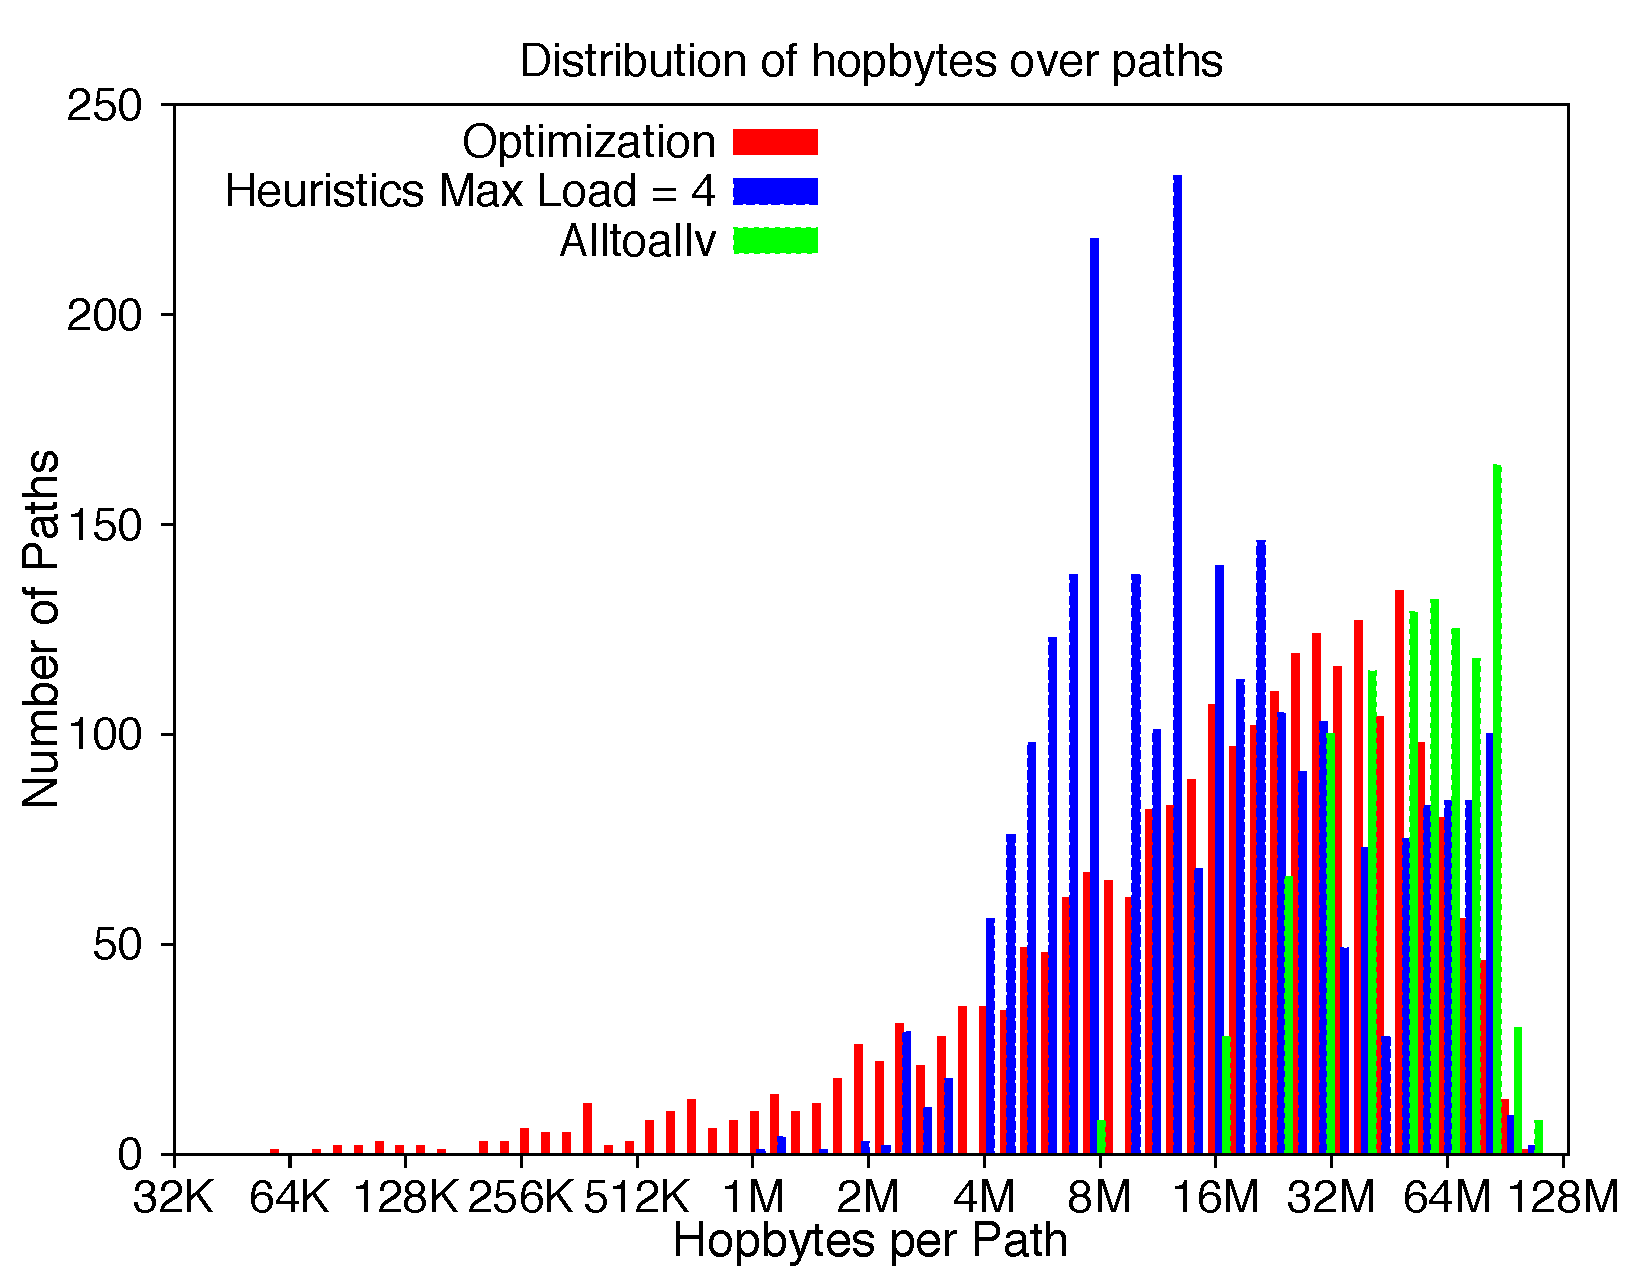
\includegraphics[width=\textwidth]{report_figures/constantr/87_2048/hopbyte_histo.pdf}
                \caption{Distribution of hopbytes over paths}
                \label{fig:87_2048_hopbyte}
        \end{subfigure}
        ~ %add desired spacing between images, e. g. ~, \quad, \qquad, \hfill etc.
          %(or a blank line to force the subfigure onto a new line)
        \begin{subfigure}[b]{0.49\textwidth}
                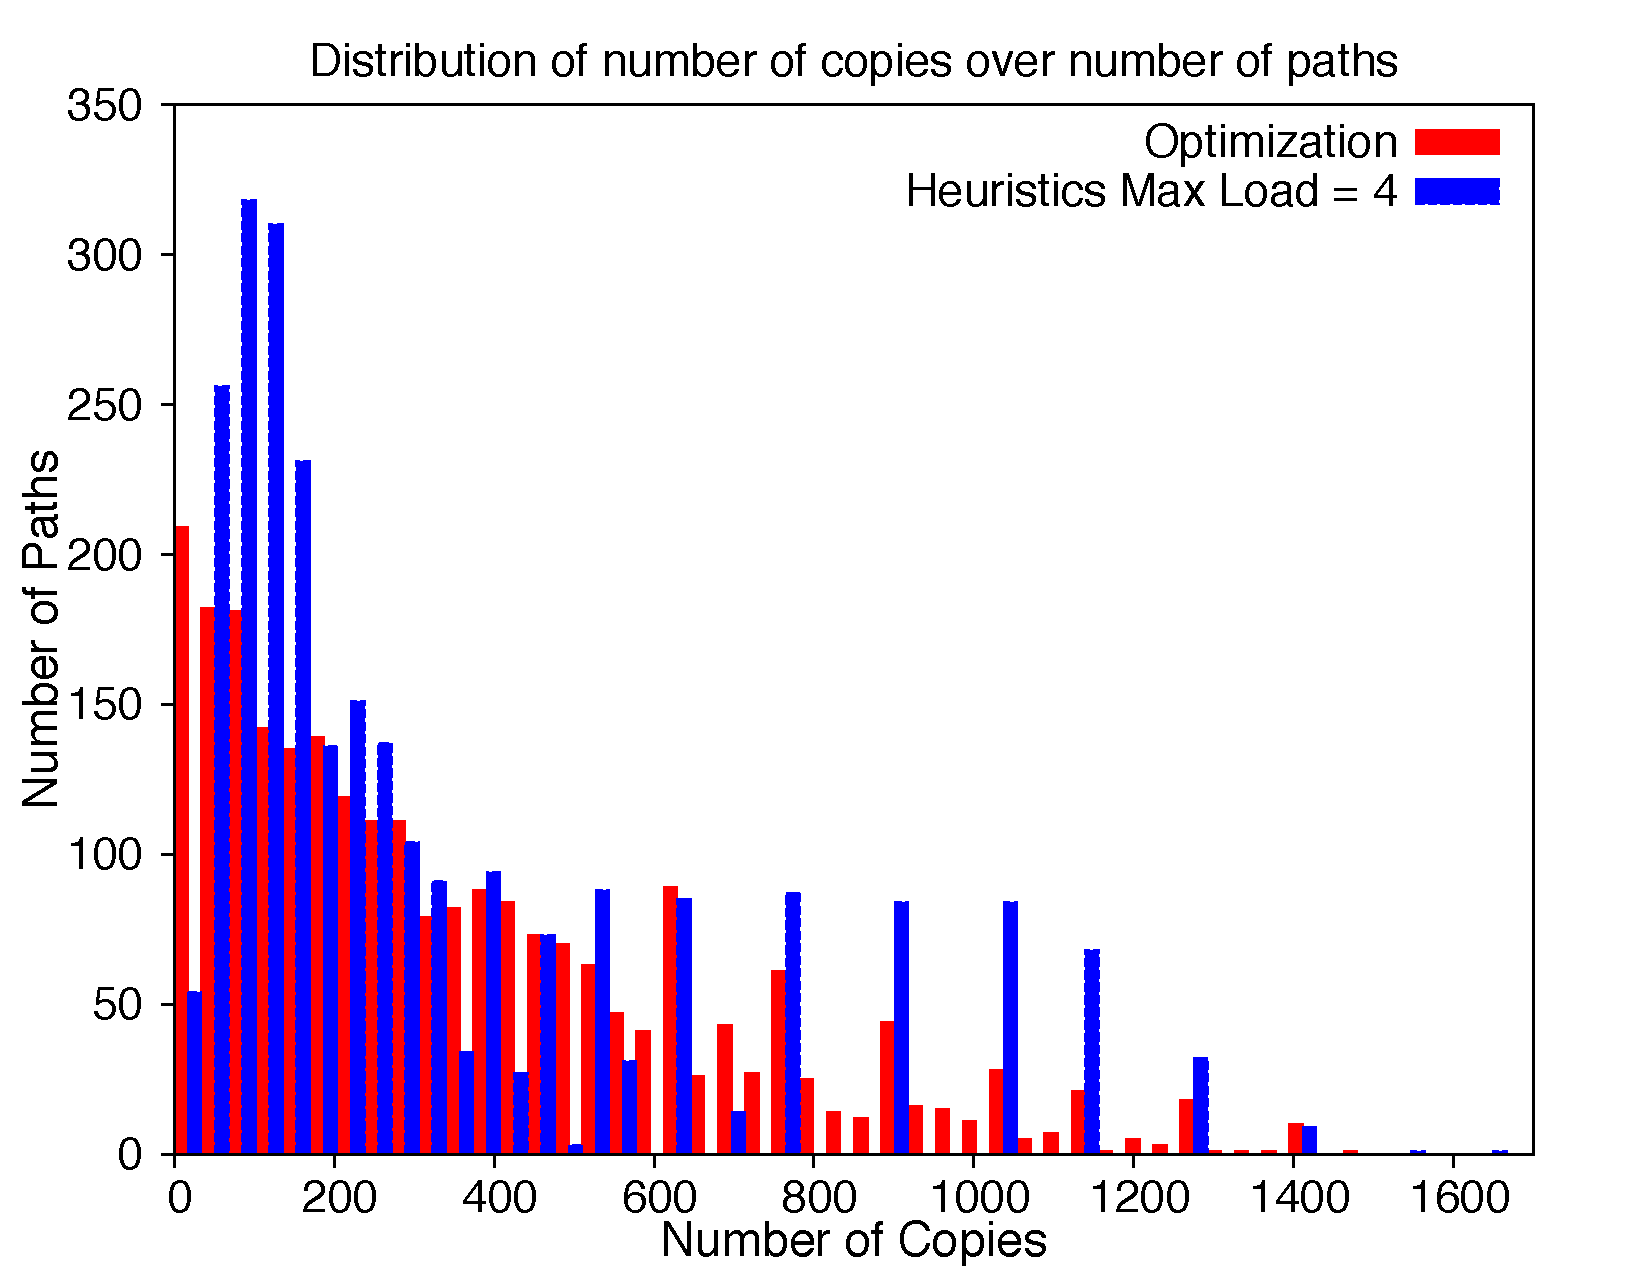
\includegraphics[width=\textwidth]{report_figures/constantr/87_2048/hopcopy_histo.pdf}
                \caption{Distribution of number of copies over paths}
                \label{fig:87_2048_hopcopy}
        \end{subfigure}
        \caption{Historgram of hops, copies, load in terms of number of paths and data size}
        \label{fig:87_2048_histo}
\end{figure}

